\documentclass[5pt]{article}
\usepackage{multicol,multirow}
\usepackage{graphicx} % Required for inserting images
\usepackage[margin=0.75cm]{geometry}
\usepackage{xcolor}
\usepackage{amsmath,esint}
\usepackage{mathtools}
\usepackage{relsize}
\usepackage{mathtools}
\usepackage{nccmath}
\usepackage[inline]{enumitem}
\usepackage{algpseudocode}

\usepackage{empheq}
\usepackage{amsfonts}

\usepackage{tkz-euclide}
\usepackage{tikz}

\definecolor{LightGray}{gray}{0.9}

\usepackage{minted}

\newenvironment{amatrix}[1]{%
  \left[\begin{array}{@{}*{#1}{c}|c@{}}
}{%
  \end{array}\right]
}

\DeclarePairedDelimiter\abs{\lvert}{\rvert}%
\DeclarePairedDelimiter\norm{\lVert}{\rVert}%
\newcommand{\universalSet}{\mathbb{U}}

\makeatletter
\let\oldabs\abs
\def\abs{\@ifstar{\oldabs}{\oldabs*}}

\newcommand{\tr}[3]{
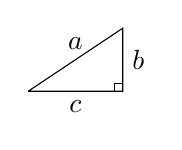
\begin{tikzpicture}[scale=0.40]
    \coordinate [] (A) at (-1.5cm,-1.cm);
    \coordinate [] (C) at (1.5cm,-1.0cm);
    \coordinate [] (B) at (1.5cm,1.0cm);
    \draw (A) -- node[above] {$a$} (B) -- node[right] {$b$} (C) -- node[below] {$c$} (A);
    \draw (1.25cm,-1.0cm) rectangle (1.5cm,-0.75cm);
\end{tikzpicture}
}


\begin{document}

\newtheorem{theorem}{Theorem}
\newtheorem{properties}{Properties}
\newtheorem{axiom}{Axiom}


\begin{center}
     \Large{\textbf{Discrete Mathematics}}\\
     \small{Class: MATH 2410}\hfill\small{\textcopyright Maximilien Notz \the\year{}}
     \noindent\rule{20.2cm}{0.4pt}
\end{center}


\begin{multicols}{2}
\setcounter{secnumdepth}{0}


\subsection{Naive Set Theory}
\subsubsection{Set Notation}
\begin{tabular}{ll}
    Universal set           & $\universalSet$\\
    Empty set               & $\emptyset=\{\}$, Remember: $\forall A (\emptyset\subset A)$\\
    Power set               & $\mathcal{P}(A)$ is the set of all the subsets of $A$.\\
    Partition of $A$        & A collection of nonempty, \small{pairwise-disjoint}\\
                            & subsets whose union is $A$.\\
    Element of              & $\in$. Example:$2\in\{1,2,3\}$\\
    Subset of               & $\subseteq$. Example: $\{A, B,C\}\subseteq\{B,C,D\}$\\
                            & $A\subseteq B \Leftrightarrow\forall x$\\
    Proper subset of        & $\subset$. Example: $\{A, B,C\}\subset\{A, B,C,D\}$\\
    Intersection            & $\bigcap_{i\in I}A_i=\{x\in\universalSet|\forall i\in I, x\in A_i\}$\\
                            & $A\cap B=\{x\in\universalSet|x\in A\land x\in B\}$\\
    Union                   & $\bigcup_{i\in I}A_i=\{x\in\universalSet|\exists i\in I, x\in A_i\}$\\
                            & $A\cup B=\{x\in\universalSet|x\in A\lor x\in B\}$\\
    Difference              & $A\backslash B=\{x\in A|x\notin B\}$\\
    Symmetric difference    & $A\Delta B=(A\backslash B)\cup(B\backslash A)$\\
    Cartesian Product       & $A\times B=\{(x,y)|x\in A\land y \in B\}$\\
    Complement of           & $A^C=\bar{A}=\{x\in\universalSet|x\notin A\}$\\
\end{tabular}

\subsubsection{Cardinality}
\begin{tabular}{ll}
    Cardinality($|A|$)  & The number of elements in a set.\\
    finite set          & Let $X$ be a finite set then $|X|\in \mathbb{N}$\\
    countable set       & A set $S$ is countable if and only if that is\\
                        & finit or $|S|=|\mathbb{N}|$.\\
    aleph null.         & $\aleph_0=|\mathbb{N}|$\\
\end{tabular}

\begin{axiom}[Axiom of extensionality]
    Two sets are equal if and only if they have the same elements.
\end{axiom}

\begin{theorem}
    Let $A$ and $B$ be sets, then $|A|=|B|$ if and only if there is a one-to-one correspondence from $A$ to $B$.
\end{theorem}

\begin{theorem}
    If $A$ and $B$ are countable, then $A\cup B$ is countable. 
\end{theorem}

\begin{theorem}[Cantor's Theorem]
    For every set $A$, $|A|<|\mathcal{P}(A)|$.
\end{theorem}

\begin{theorem}[Schr\"oder--Bernstein]
     If there are injective function(one-to-one) functions $f\!:A\to B$ and $g\!:B\to A$, then there is a one-to-one correspondence between $A$ and $B$. 
     In other words If $A$ and $B$ are set with $|A|\neq|B|$ and $|B|\neq|A|$, then $|A|=|B|$.
\end{theorem}

\begin{theorem}[Well-Ordering Principle]
    Every nonempty subset of $\mathbb{N}$ has a least element.
\end{theorem}

\begin{properties}
    Let $S$ be the universal set.
    \begin{itemize*}
        \item if $A\subseteq B$ and $B\subseteq A$ then  $A=b$.
        \item $\forall A, A\subseteq A$
        \item $|\mathcal{P}(A)|=2^{|A|}$
        \item $A\cup A=A\cap A=A$
        \item $A\cup\emptyset=A$
        \item $A\cap\emptyset=\emptyset$
        \item $A\cup S=S$ 
        \item $A\cap S=A$
        \item $(A\cup B)\cup C=A\cup (B\cup C)$
        \item $(A\cap B)\cap C=A\cap (B\cap C)$
        \item $A\cup B =B\Leftrightarrow A\subseteq B$
        \item $A\cup B =A\Leftrightarrow A\subseteq B$
        \item $A\backslash B \neq B\backslash A$
        \item $A\backslash\emptyset = A$
        \item $A\backslash S=\emptyset$
        \item $A\backslash\emptyset =A\Leftrightarrow A\subseteq B$
        \item $A\backslash S= A^C$
        \item $A\times (B\cup C) = (A\times B)\cup (A\times C)$
        \item $ A\cap (B\cup C)=(A\cap B)\cup(A\cap C)$
        \item $(A\cup B)^C=A^C\cap B^C$
        \item $(A\cap B)\backslash C =(A\backslash C)\cap(B\backslash C)=A\cap(B\backslash C)$
        \item $A\backslash (B\cap C)=(A\backslash B)\cup (A\backslash C)$
    \end{itemize*}
\end{properties}

\subsection{Functions}

\begin{tabular}{ll}
    Functions           & A rule that assigns each input exactly one \\
                        & output.\\
    Domain              & The set of all input of a function.($X$ in $f:X\rightarrow Y$)\\
    Codomain            & The set of all output a function.($Y$ in $f:X\rightarrow Y$)\\
    Range               & Is the subset of Y of elements that have an\\
                        & antecedent in X by f\\
    $f:x\rightarrow y$  & a function $f$ with a domain $x$ and a codomain $y$.\\
    Recursive f.        & \\
    Injective           & every element of the codomain is the image  of \\
                        & $f(a)=f(b)\Rightarrow a=b$\\
                        & \textbf{at most} one element from the domain.\\
    Surjective          & every element of the codomain is the image  of \\
                        & \textbf{at least} one element from the domain.\\
    Bijection           & A function that is \textbf{Injective} and \textbf{Surjective}.\\
    Image               & $f(A)=\{f(a)\in Y: a\in A\}$, where $A\subset\text{domain}$.\\
    Inverse Image       & $f^{-1}(B)=\{f(b)\in X: b\in B\}$, where \\
                        & $B\subset\text{codomain}$.\\
    Set of Function     & $B^A$ contains all functions from $A$ to $B$ ($A\rightarrow B$).\\
\end{tabular}

\subsection{Counting}

\begin{tabular}{ll}
    n-bit string            & \\
    bit string weight       & the number of \textbf{1} in a bit string.\\
    $\bf{B}^n_k$            & the set of all \textbf{n-bit strings} of weight k.\\
    Factorial               & $n!=n\cdot(n-1)\cdot(n-2)\cdot...\cdot 1$\\
\end{tabular}

\subsubsection{Additive Principle}
\textbf{General Definition:} 
if event $A$ can occur in $m$ ways, and even $B$ can occur in $n$ \textbf{disjoint} ($A$ and $B$ can't apen at the same time.) ways, then $A$ and $B$ can occur in $m+n$ ways.\\   
\textbf{Set Definition:} Given 2 sets $A$ and $B$, then $|A\cup B| = |A| + |B| - |A\cap B|$. Given 3 sets $A$, $B$ and $C$, then $|A\cup B\cup C| = |A| + |B| + |C| - |A\cap B| - |A\cap C|- |C\cap B|+|A\cap B\cap C|$.


\subsubsection{Multiplicative Principle}
\textbf{General Definition:} if event $A$ can occur $m$ ways, and each possibility for $A$ allows for exactly $n$ ways for event $B$, then the event "$A$ and $B$" can occur $m\cdot n$ ways.\\
\textbf{Set Definition:} Given 2 sets $A$ and $B$, we have $|A\times B|=|A|\cdot|B|$.

\subsubsection{Permutations}
\textbf{Definition:} Ordered selections of $k$ distinct elements drawn from an $n$-element set.\\
\begin{itemize*}
    \item Without repetition: $P(n,k)=\dfrac{n!}{(n-k)!}$.
    \item With repetition of symbols allowed from an alphabet of size $m$: $m^k$ length-$k$ strings.
\end{itemize*}

\subsubsection{Combinations}
\textbf{Definition:} Unordered selections of $k$ elements from an $n$-element set.\\
\begin{itemize*}
    \item Without repetition: $C(n,k)=\binom{n}{k}$.
    \item With repetition allowed: $C_{\text{rep}}(n,k)=\binom{n+k-1}{k}$.
\end{itemize*}

\subsubsection{Binomial coefficient}
\textbf{Formula:} $n \text{ choose } k=\binom{n}{k}=\frac{n!}{(n-k)!k!}$
\begin{theorem}[Binomial Theorem]
    $(a+b)^n=\sum^n_{k=0}\binom{n}{k}a^{n-k}b^k$
\end{theorem}
\begin{properties}
    \begin{itemize*}
        \item $\binom{n}{k}$ is the number of subset of size $n$ each of cardinality $k$.
        \item $\binom{n}{k}=\binom{n-1}{k-1}+\binom{n-1}{k}$
        \item $\binom{n}{k}=|\bf{B}^n_k|$
        \item $\sum_{k=0}^{n}\binom{n}{k}=2^n$
    \end{itemize*}
\end{properties}

\subsection{Symbolic Logic}
\begin{tabular}{lcl}
    \textbf{Name}           & \textbf{Symbol}               & \textbf{Translate to}\\
    Conjunction             & $A\land B$                    & $A$ and $B$.\\
    Disjonction             & $A\lor B$                     & $A$ or $B$.\\
    Negation                & $\lnot A$                     & not $A$.\\
    Condition/Implication   & $A\Rightarrow B$              & if $A$ then $B$.\\
    Bicondition             & $A\Leftrightarrow B$          & if and only if $A$ then $B$.\\
    Exclusive Disjunction   & $A\oplus B$                   & Either $A$ or $B$, but not both.\\
    Universal               & $\forall x$                   & For all $x$'s.\\
    Existential             & $\exists x$                   & There is at least one $x$.\\
    Unique Existential      & $\exists! x$                  & There is exactly one $x$.\\
    Equivalence             & $A\equiv B$                   & $A$ is identical to $B$.\\
\end{tabular}
\textbf{Converse:} $B\Rightarrow A$ is the converse of $A\Rightarrow B$.\\
\textbf{Contrapositive:} $\lnot B\Rightarrow \lnot A$ is the Contrapositive of $A\Rightarrow B$. 

\subsubsection{Important Equivalences \& Properties}
\begin{itemize*}
    \item $\lnot(\lnot A)\equiv A$
    \item $p\land T\equiv p$
    \item $p\land\bot\equiv\bot$
    \item $p\lor T\equiv T$
    \item $p\lor\bot\equiv p$
    \item $A\oplus B\equiv (A\lor B)\land\lnot(A\land B)$
    \item $p\Rightarrow q\equiv \lnot q\Rightarrow \lnot p$
    \item $p\Rightarrow q\equiv \lnot p \lor q$
    \item $p\Leftrightarrow q\equiv (p\Rightarrow q)\land(q\Rightarrow p)$
    \item $\lnot (p\Leftrightarrow q)\equiv \lnot p \Leftrightarrow q\equiv p \Leftrightarrow \lnot q$
    \item $\lnot B\Rightarrow \lnot A \equiv A\Rightarrow B$
\end{itemize*}

\begin{properties}
    \begin{itemize*}
        \item $A\lor B\equiv B\lor A$
        \item $A\lor (B\lor C)\equiv C\lor (A\lor B)$
        \item $A\land B\equiv B\land A$
        \item $A\land(B\land C)\equiv C\land (A\land B)$
        \item $A\oplus B\equiv B\oplus A$
        \item $A\oplus(B\oplus C)\equiv C\oplus (A\oplus B)$
    \end{itemize*}
\end{properties}

\subsubsection{deMorganLaws}
\begin{itemize*}
    \item $\lnot\forall xP(x)=\exists xP(\lnot x)$
    \item $\lnot\exists xP(x)=\forall xP(\lnot x)$
    \item $\lnot\exists x\exists yP(x,y)=\forall x\exists yP(\lnot x,y)$
    \item $\lnot\left(\bigwedge_{i=0}^na_i\right)\equiv\bigvee_{i=0}^n\lnot a_i$
    \item $\lnot\left(\bigvee_{i=0}^na_i\right)\equiv\bigwedge_{i=0}^n\lnot a_i$
\end{itemize*}


\subsection{Proofs}
\subsubsection{Rules of inference}
\begin{tabular}{ll}
    Modus Ponens            &   If $p\Rightarrow q$ and $p$, then $q$.\\
    Modus Tollens           &   If $p\Rightarrow q$ and $\lnot q$, then $\lnot p$.\\
    Hypothetical Syllogism  &   If $p\Rightarrow q$ and $q\Rightarrow R$, then $p\Rightarrow r$.\\
    Disjunctive Syllogism   &   If $p\lor q$ and $\lnot q$, then $p$.\\
    Addition                &   If $p$, then $p\lor q$.\\
    Simplification          &   If $p\land q$, then $p$.\\
    Conjuction              &   If $p$ and $q$, then $p\land q$.\\
    Absorption              &   If $p\Rightarrow q$, then $p\Rightarrow (p\land q)$.\\
    Resolution              &   If $P\lor Q$ and $\lnot P\lor R$, then $Q\lor R$.
\end{tabular}

\subsubsection{Direct Proof}
\textbf{Goal:} Prove $p\Rightarrow q$.\\
\textbf{Idea:} Assume $p$ and use definitions/algebra to derive $q$.\\

\subsubsection{Proof by Contrapositive}
\textbf{Goal:} Prove $p\Rightarrow q$.\\
\textbf{Idea:} Instead of proving $p\Rightarrow q$, prove $\lnot q\Rightarrow \lnot p$.\\

\subsubsection{Proof by Counter Example}
\textbf{Goal:} Disprove $\forall x\,P(x)$ (show $\exists x\,\lnot P(x)$).\\
\textbf{Idea:} Exhibit a specific counterexample $x_0$ with $\lnot P(x_0)$.\\

\subsubsection{Proof by Cases}
\textbf{Goal:} Prove the claim.\\
\textbf{Idea:} Split into exhaustive, mutually exclusive cases and prove the claim in each case.\\

\subsubsection{Proof by Contradiction}
\textbf{Goal:} Prove a statement $S$.\\
\textbf{Idea:} Assume $\lnot S$ and derive a contradiction; conclude $S$.\\

\subsubsection{Proof by Mathematical Induction}
\textbf{Goal:} Prove $\forall n\ge n_0,\;P(n)$.\\
\textbf{Base Case:} Verify $P(n_0)$ (and additional initial values if required).\\
\textbf{Inductive Step:} Assume $P(k)$ holds for an arbitrary $k\ge n_0$ (inductive hypothesis) and show $P(k+1)$ holds.\\
\textbf{Conclusion:} If both steps succeed, the principle of mathematical induction yields $P(n)$ for all $n\ge n_0$.\\

\subsubsection{Proof by Strong Induction}
\textbf{Goal:} Prove $\forall n\ge n_0,\;P(n)$.\\
\textbf{Base Case(s):} Establish $P(n_0),P(n_0+1),\dots,P(n_0+r)$ as needed.\\
\textbf{Inductive Step:} Assume $P(n_0),P(n_0+1),\dots,P(k)$ all hold (strong hypothesis) and deduce $P(k+1)$.\\
\textbf{Conclusion:} By strong induction, $P(n)$ holds for every $n\ge n_0$.\\

\subsection{Graphs}
A \textbf{graph} is an ordered pair \boxed{$G=(V,E)$}, where $V$ is a nonempty set of \textbf{vertices} and $E$ is a nonempty set of \textbf{edges}.\\
\begin{tabular}{ll}
    Vertices & \\
    edges    & \\
    adjacent & if 2 edges are connected by a vertice.\\
    isomorphism & \\
    isomorphic  & if there is an isomorphism between 2 graphs.\\
    
\end{tabular}

\end{multicols}
\end{document}
